\chapter{Unidad 6. Gestión de la memoria principal}
La memoria principal, o memoria RAM (Random Access Memory), es un componente esencial en los sistemas informáticos. 
Almacena temporalmente los datos y programas que están en ejecución o listos para ser ejecutados por la CPU (Unidad Central de Procesamiento). A diferencia de la memoria secundaria, la memoria principal permite un acceso rápido y directo, lo cual es crucial para el rendimiento y eficiencia del sistema.
\section{
	Direccionamiento
}
El direccionamiento se refiere al proceso mediante el cual el sistema operativo y el hardware de la computadora determinan y gestionan las ubicaciones de memoria donde se almacenan los datos e instrucciones. Este proceso involucra la asignación y la manipulación de direcciones de memoria que se utilizan para acceder a los datos que un proceso necesita durante su ejecución.

Existen \textbf{dos tipos de direccionamiento:}
\begin{itemize}
	\item \textbf{Direccionamiento físico:} Corresponden a ubicaciones reales en la memoria RAM. Son las direcciones que utiliza el hardware para acceder a los datos almacenados.
	\item \textbf{Direccionamiento lógico:} Son generadas por la CPU y utilizadas por los programas en ejecución. Representan una abstracción de la memoria física y permiten que cada proceso tenga su propio espacio de direcciones.
\end{itemize}
\begin{figure}[H] \centering 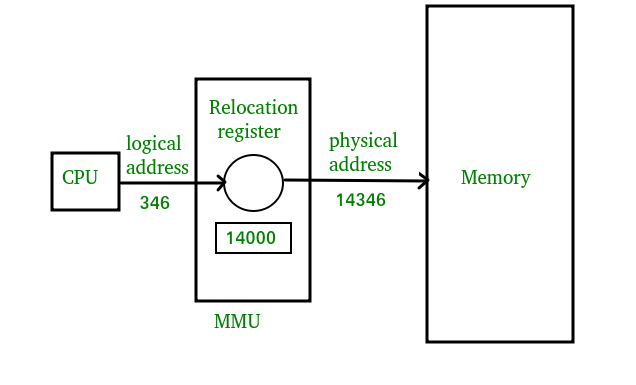
\includegraphics[width=0.6\linewidth]{Imagenes/direccionamiento.png} \caption{El procesador genera direcciones lógicas, mientras que la memoria RAM, contiene direcciones físicas.} \end{figure}

\subsection{Asignación de direcciones por MMU}

En el contexto de la gestión de la memoria principal, el direccionamiento se refiere al proceso mediante el cual el sistema operativo y el hardware de la computadora determinan y gestionan las ubicaciones de memoria donde se almacenan los datos e instrucciones. Este proceso involucra la asignación y la manipulación de direcciones de memoria que se utilizan para acceder a los datos que un proceso necesita durante su ejecución.

\begin{figure}[H] \centering 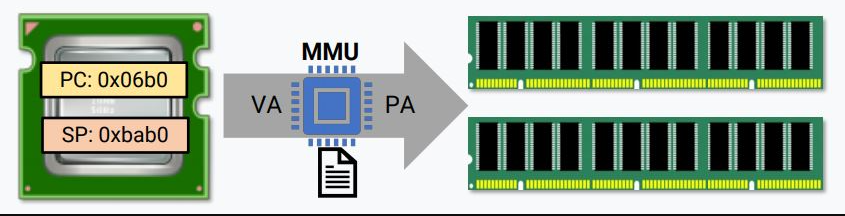
\includegraphics[width=0.6\linewidth]{Imagenes/mmu.png} \caption{La unidad MMU gestiona las ubicaciones de memoria.} \end{figure}


 \section{Jerarquía de almacenamiento}
La jerarquía de almacenamiento es un modelo que organiza los distintos tipos de memoria en un sistema computacional, incluyendo tanto la memoria volátil (RAM, caché, registros) como la memoria no volátil (discos duros, SSD), en niveles jerárquicos. Se basa en tres criterios principales: velocidad, costo y capacidad. Cada nivel de la jerarquía tiene características diferentes, con las memorias más cercanas a la CPU siendo más rápidas pero más costosas y de menor capacidad, mientras que las me

\begin{figure}[H] \centering 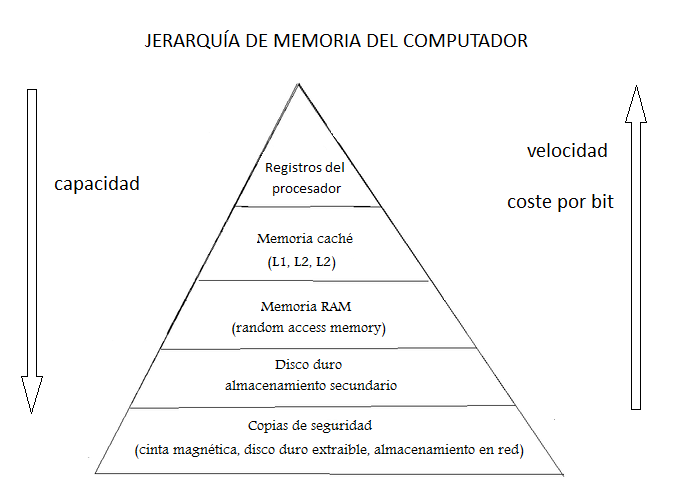
\includegraphics[width=0.6\linewidth]{Imagenes/coste.png} \caption{En la jerarquía de almacenamiento,  la capacidad es inversamente proporcional  a la velocidad y coste.} \end{figure}

\subsection{Niveles de jerarquía de almacenamiento}
En la figura anterior se muestran los diferentes niveles de la jerarquía de almacenamiento. A medida que se asciende en la pirámide, se aumenta la velocidad de acceso, pero se reduce la capacidad y el costo por bit es mayor. A continuación se describe cada nivel de manera detallada:


 \begin{tcolorbox}[title= Níveles de almacenamiento]
	\begin{itemize}
		
		
		\item \textbf{Registros:}
		Los registros están ubicados dentro del núcleo del CPU. Son la memoria más cercana al procesador, con capacidad muy limitada (solo unos pocos bytes), pero su acceso es el más rápido de todo el sistema. Los registros se utilizan para almacenar datos temporales y resultados inmediatos que se requieren para ejecutar instrucciones rápidamente.
		\item \textbf{Memoria caché:}
		La memoria caché también está ubicada dentro del procesador y se organiza en varios niveles: L1, L2 y L3. La caché L1 es la más rápida y cercana al núcleo del procesador, pero también la más pequeña. La caché L2 es más grande y ligeramente más lenta, mientras que la caché L3 es compartida entre todos los núcleos de la CPU, permitiendo que la comunicación entre estos sea más eficiente. La memoria caché almacena datos e instrucciones que se utilizan con frecuencia, reduciendo así la necesidad de acceder a la memoria RAM.
		\item \textbf{Memoria RAM:}
		La memoria RAM es la memoria volátil donde se cargan los programas y datos que están siendo utilizados activamente por el sistema. Aunque la RAM ha alcanzado grandes capacidades de almacenamiento en los sistemas modernos, su contenido se pierde cuando el equipo se apaga. Es más lenta que la caché, pero mucho más rápida que el almacenamiento secundario, y es esencial para la ejecución eficiente de programas.
		\item \textbf{Almacenamiento Secundario:}
		El almacenamiento secundario incluye dispositivos como discos duros (HDD) y unidades de estado sólido (SSD), que se utilizan para almacenar datos y programas de manera permanente. Los discos duros tradicionales (HDD) son más lentos y más baratos por bit, pero ofrecen grandes capacidades de almacenamiento. Las SSD, aunque más rápidas, son más costosas por bit y suelen tener capacidades menores en comparación con los HDD. El acceso a esta memoria es mucho más lento que en la RAM, pero su gran capacidad la hace ideal para almacenar grandes volúmenes de datos.
		
	\end{itemize}
\end{tcolorbox}



\section{Gestión de la memoria}
La gestión de la memoria es una función del sistema operativo que administra la memoria principal (RAM). Podemos establecer que el gestor de memoria:

\begin{itemize}
	\item Asigna y libera memoria a los procesos.
	\item Hace un seguimiento sobre el uso de la memoria para evitar conflictos.
	\item Optimiza el rendimiento asegurando el uso eficiente de la memoria.
\end{itemize}

El gestor de memoria es fundamental para garantizar un uso adecuado de la memoria, proporcionando una base sólida para las distintas técnicas de gestión que permiten la coexistencia de procesos en la memoria principal.

Para optimizar la gestión de la memoria, se utilizan técnicas como la monoprogramación y la multiprogramación, que permiten administrar de manera más eficiente el uso de la memoria según las necesidades del sistema.

\subsection{Monoprogramación}
La monoprogramación permite ejecutar un solo proceso a la vez. Toda la memoria principal se asigna al proceso en ejecución.

\begin{itemize}
	\item \textbf{Memoria dedicada: }Toda la memoria se asigna a un único proceso, sin interferencias. Esto es simple, pero ineficiente si el proceso no usa toda la memoria.
	\item \textbf{Monitor residente: }Parte del sistema operativo siempre reside en la memoria para gestionar tareas básicas, lo que reduce la memoria disponible para el proceso.
\end{itemize}

\textbf{Ventajas}: Simplicidad y fácil gestión.

\textbf{Desventajas}: Uso ineficiente del CPU y la memoria, ya que solo se ejecuta un proceso a la vez.

\subsection{Multiprogramación}
 La multiprogramación permite que varios procesos residan en la memoria al mismo tiempo, maximizando el uso del CPU.
 
 \begin{itemize}
 
 	\item \textbf{Particiones de la memoria:}
 	\begin{itemize}
 		\item\textbf{ Fijas: }Se dividen en secciones de tamaño fijo. Es simple, pero puede generar fragmentación interna.
 		\item \textbf{Variables: }Se ajustan al tamaño del proceso. Reducen la fragmentación interna, pero pueden generar fragmentación externa.
 	\end{itemize}
 		\item \textbf{Protección de la memoria: }Cada proceso tiene acceso solo a su propia porción de memoria, garantizado por registros de base y límite que son verificados por la MMU.
 	\item \textbf{Algoritmos de asignación:}
 	\begin{itemize}
 		\item First-Fit: Asigna la primera porción libre suficientemente grande.
 		\item Best-Fit: Asigna la porción más cercana al tamaño solicitado.
 		\item Worst-Fit: Asigna la mayor porción libre disponible.
 	\end{itemize}
 \end{itemize}
 
 \textbf{Ventajas}: Mejora la utilización del CPU al ejecutar múltiples procesos. La CPU cambia a otro proceso cuando uno está en espera.
 

 
 
 
\subsection{Segmentación}

La segmentación es una técnica de gestión de la memoria que se enfoca en el punto de vista del usuario. En lugar de dividir la memoria en particiones físicas arbitrarias, la segmentación la divide en segmentos lógicos, cada uno de los cuales corresponde a una parte específica del programa o a un tipo de dato, como el código, la pila o las variables globales.

\begin{figure}[H] \centering 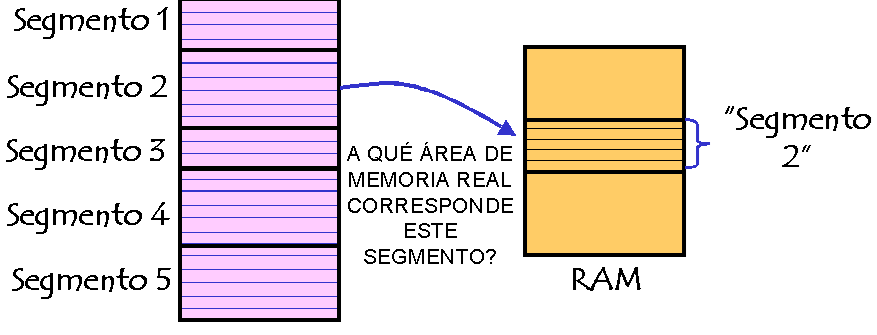
\includegraphics[width=0.6\linewidth]{Imagenes/segmentacion.png} \caption{Esquema de segmentación]} \end{figure}


\begin{itemize}
	\item Segmentos Lógicos: Cada programa se divide en segmentos lógicos, como el código, la pila, y las variables globales. Cada segmento tiene una función específica, lo que facilita la gestión de la memoria desde una perspectiva más intuitiva para el usuario.
	\item Tabla de Segmentos: El sistema operativo mantiene una tabla de segmentos para cada proceso. Esta tabla almacena la dirección base y el tamaño de cada segmento, que se utilizan para traducir las direcciones lógicas a físicas.
	\item Ventaja para el Usuario: La segmentación permite mayor flexibilidad al gestionar las diferentes partes del programa de manera independiente. Además, facilita la protección de la memoria, ya que cada segmento puede tener permisos de acceso específicos.
\end{itemize}

	


 \subsection{Memoria Virtual}
La memoria virtual es una técnica avanzada que permite a los sistemas operativos ejecutar programas que requieren más memoria de la que está físicamente disponible en la RAM. Esta técnica combina la memoria principal (RAM) con el almacenamiento secundario (disco duro o SSD) para crear una "memoria extendida" que da la impresión de tener una gran cantidad de memoria disponible.

\begin{itemize}

	
	\item \textbf{Swapping}: Cuando la memoria principal está llena, el sistema operativo utiliza el  \textbf{swapping} para intercambiar páginas activas de la RAM con páginas almacenadas en el disco. Esto permite liberar espacio en la memoria principal para otros procesos.
	
\end{itemize}
 